\documentclass[11pt,a4paper]{scrartcl}

% language
\usepackage[utf8]{inputenc}
\usepackage[ngerman]{babel}	% Deutsches Paket

% Math
\usepackage{amsmath}
\usepackage{amssymb}
\usepackage{amsthm}

%tables
\usepackage{multirow}

% graphics
\usepackage[usenames,dvipsnames]{color}	
\usepackage{xcolor}	
\definecolor{gray}{rgb}{0.96,0.96,0.96}
\definecolor{ngray}{rgb}{0.16,0.16,0.8}
\definecolor{shell_key}{HTML}{333399}
\usepackage{graphicx}
\usepackage{float}
\usepackage{tikz}
\usetikzlibrary{arrows,matrix,shapes,trees}

% conding
\usepackage{listings}
\usepackage{microtype}
\usepackage{caption}

% Shell environment
\newcounter{cntShell}
\newcommand{\lstShell}[1][]{
	\renewcommand*\lstlistingname{Shell}
	\lstset{style=shell}
	\ifthenelse
		{\isempty{#1}}
		{\lstset{title={},caption={}}}
		{
			\stepcounter{cntShell}
			\lstset{title={\lstlistingname\ \arabic{cntShell}: #1}}
		}
}
\lstdefinestyle{shell}{
	language=bash,
	basicstyle=\ttfamily,
    keywordstyle=\color{blue}\ttfamily,
    stringstyle=\color{red}\ttfamily,
    commentstyle=\color{OliveGreen}\ttfamily,
	numbersep=5pt,
	backgroundcolor=\color{gray},
	showspaces=false,
	tabsize=2,
	breaklines=true,
	prebreak={\textbackslash},
	literate={\$}{{\textcolor{shell_key}{\$}}}1,
	literate={\\\#}{{\textcolor{black}{\#}}}1,
	morekeywords={apropos,cp,df,du,ls,man,mkdir,mount,mv,rm,touch,umount,wc}
}

% Bash environment
\newcounter{cntBash}
\newcommand{\lstBash}[1][]{
	\renewcommand*\lstlistingname{Bash}
	\lstset{style=bash}
	\ifthenelse
		{\isempty{#1}}
		{\lstset{title={},caption={}}}
		{
			\stepcounter{cntBash}
			\lstset{title={\lstlistingname\ \arabic{cntBash}: #1}}
		}
}
\lstdefinestyle{bash}{
	language=bash,
	basicstyle=\ttfamily,
    keywordstyle=\color{blue}\ttfamily,
    stringstyle=\color{red}\ttfamily,
    commentstyle=\color{OliveGreen}\ttfamily,
	numbersep=5pt,
	backgroundcolor=\color{gray},
	showspaces=false,
	tabsize=2,
	breaklines=true,
	prebreak={\textbackslash},
	literate={\\\$}{{\$}}1,
	morekeywords={in,esac}
}

% C environment
\newcounter{cntCcode}
\newcommand{\lstCcode}[1][]{
	\renewcommand*\lstlistingname{C-Code}
	\lstset{style=ccode}
	\ifthenelse
		{\isempty{#1}}
		{\lstset{title={},caption={}}}
		{
			\stepcounter{cntCcode}
			\lstset{title={\lstlistingname\ \arabic{cntCcode}: #1}}
		}
}
\lstdefinestyle{ccode}{
	language=C++,
	basicstyle=\ttfamily,
    keywordstyle=\color{blue}\ttfamily,
    stringstyle=\color{red}\ttfamily,
    commentstyle=\color{OliveGreen}\ttfamily,
	numbersep=5pt,
	backgroundcolor=\color{gray},
	showspaces=false,
	tabsize=2,
	breaklines=true,
	prebreak={\textbackslash}
}

% Haskell environment
\newcounter{cntHaskell}
\newcommand{\lstHaskell}[1][]{
	\renewcommand*\lstlistingname{Haskell}
	\lstset{style=haskell}
	\ifthenelse
		{\isempty{#1}}
		{\lstset{title={},caption={}}}
		{
			\stepcounter{cntHaskell}
			\lstset{title={\lstlistingname\ \arabic{cntHaskell}: #1}}
		}
}
\lstdefinestyle{haskell}{
	language=Haskell,
	basicstyle=\ttfamily,
    keywordstyle=\color{blue}\ttfamily,
    stringstyle=\color{red}\ttfamily,
    commentstyle=\color{OliveGreen}\ttfamily,
	numbersep=5pt,
	backgroundcolor=\color{gray},
	showspaces=false,
	tabsize=2,
	breaklines=true,
	prebreak={\textbackslash},
	literate={\\\$}{{\textcolor{black}{\$}}}1
}

% other
\usepackage{enumerate}
\usepackage{xifthen}


\makeatletter
\newenvironment{btHighlight}[1][]
{\begingroup\def\bt@Highlight@par{#1}\begin{lrbox}{\@tempboxa}}
{\end{lrbox}\bt@HL@box[\bt@Highlight@par]{\@tempboxa}\endgroup}

\newcommand\btHL[1][]{%
\begin{btHighlight}[#1]\bgroup\aftergroup\bt@HL@endenv%
}
\def\bt@HL@endenv{%
\end{btHighlight}%   
\egroup
}
\newcommand{\bt@HL@box}[2][]{%
  $\overset{\text{#1}}{\overbrace{\strut\usebox{#2}}}$%
}
\makeatother

\makeatletter
\newenvironment{bbHighlight}[1][]
{\begingroup\def\bb@Highlight@par{#1}\begin{lrbox}{\@tempboxa}}
{\end{lrbox}\bb@HL@box[\bb@Highlight@par]{\@tempboxa}\endgroup}
\newcommand\bbHL[1][]{%
\begin{bbHighlight}[#1]\bgroup\aftergroup\bb@HL@endenv%
}
\def\bb@HL@endenv{%
\end{bbHighlight}%   
\egroup
}
\newcommand{\bb@HL@box}[2][]{%
  $\underset{\text{#1}}{\underbrace{\strut\usebox{#2}}}$%
}
\makeatother

\title{Paradigmen der Programmierung}
\subtitle{Vorlesungsnotizen bis 18.06.2014 (ohne Lisp)}
\author{Felix Beuster}
\date{}

\begin{document}
\setlength{\parindent}{0ex}
\maketitle
\newpage
\tableofcontents
\newpage

\section*{Vorwort} % (fold)
\label{sec:vorwort}
\addcontentsline{toc}{section}{Vorwort}

	Hierbei handelt es sich um meine digitalisierten Mitschriften aus der Vorlesung Paradigmen der
	Programmierung. Diese Sammlung erhebt keinen Anspruch auf Vollständigkeit, Korrekturhinweise
	und Erweiterungsvorschläge seitens der Kommilitonen sind gerne gesehen.

% section vorwort (end)

\section{Shellprogrammierung} % (fold)
\label{sec:shellprogrammierung}
	

	Themen der Vorlesung:
	\begin{itemize}
		\item Shellprogrammierung
		\item Standardtools
		\item Fallstudie DZNE sensor based monitoring
	\end{itemize}

	\subsection{Shells und Tools} % (fold)
	\label{sub:shells_und_tools}

		\texttt{numbers.dat} enthält $793\cdot10^8$ Zahlen, \texttt{summary} rechnet Werte
		spaltenweise aus

		
		\lstShell[Einfache Eingabeumleitung]
		\begin{lstlisting}
$ cp summary < numbers.dat
		\end{lstlisting}

		\lstShell[1. Zeile auslassen, da bspw. Kommentar]
		\begin{lstlisting}
$ tail -1 < numbers.dat | summary
		\end{lstlisting}

		Problem bei \texttt{tail} und anderen Pipeline-Operationen:\\
		Es laufen 2 Programme,  alle Daten durchlaufen die CPU zweimal, problematisch auf
		Single Core\\

		Shell-Skript (siehe Foliensatz) besser geeignet. Aufruf dann wieder:

		\lstShell
		\begin{lstlisting}
$ buttfirst.sh < numbers.dat
		\end{lstlisting}

		Eine gesonderte Berücksichtigung der Standardeingabe/-ausgabe muss nicht durch das
		Programm erfolgen

		\subsubsection*{Fallstudie: DZNE sensor based monitoring} % (fold)
		\label{ssub:fallstudie_dzne_sensor_based_monitoring}
		% subsubsection fallstudie_dzne_sensor_based_monitoring (end)
	
	% subsection shells_und_tools (end)

	%%%%
	%%%% end V1
	%%%% % 1. VL
	

	\subsection{Prozesspipelines und Glue Languages} % (fold)
	\label{sub:prozesspipelines_und_glue_languages}
	
	Unix verfolgt das Konzept: \textbf{Alles ist eine Datei}
	\begin{flalign*}
		 \left.\begin{array}{c}
		 	\text{.c}\\
		 	\text{.java}\\
		 	\text{.f77}
		 \end{array}\right\}\text{ Compiler }\rightarrow\text{a.out}
	\end{flalign*}
	Vorteile:
	\begin{itemize}
		\item auch Kompilat braucht keine unterschiedlichen Prozeduren
		\item kein gerätespezifischer Code
	\end{itemize}
	Dateiunabhängig ist damit möglich
	\lstCcode[Lies aus Datei 1 1 Byte und speicher es in c]
	\begin{lstlisting}
read(1,1,&c);
	\end{lstlisting}

	\begin{figure}[hb]
		\caption{Schnittstellen auf System-Ebene zu Abstraktion}
		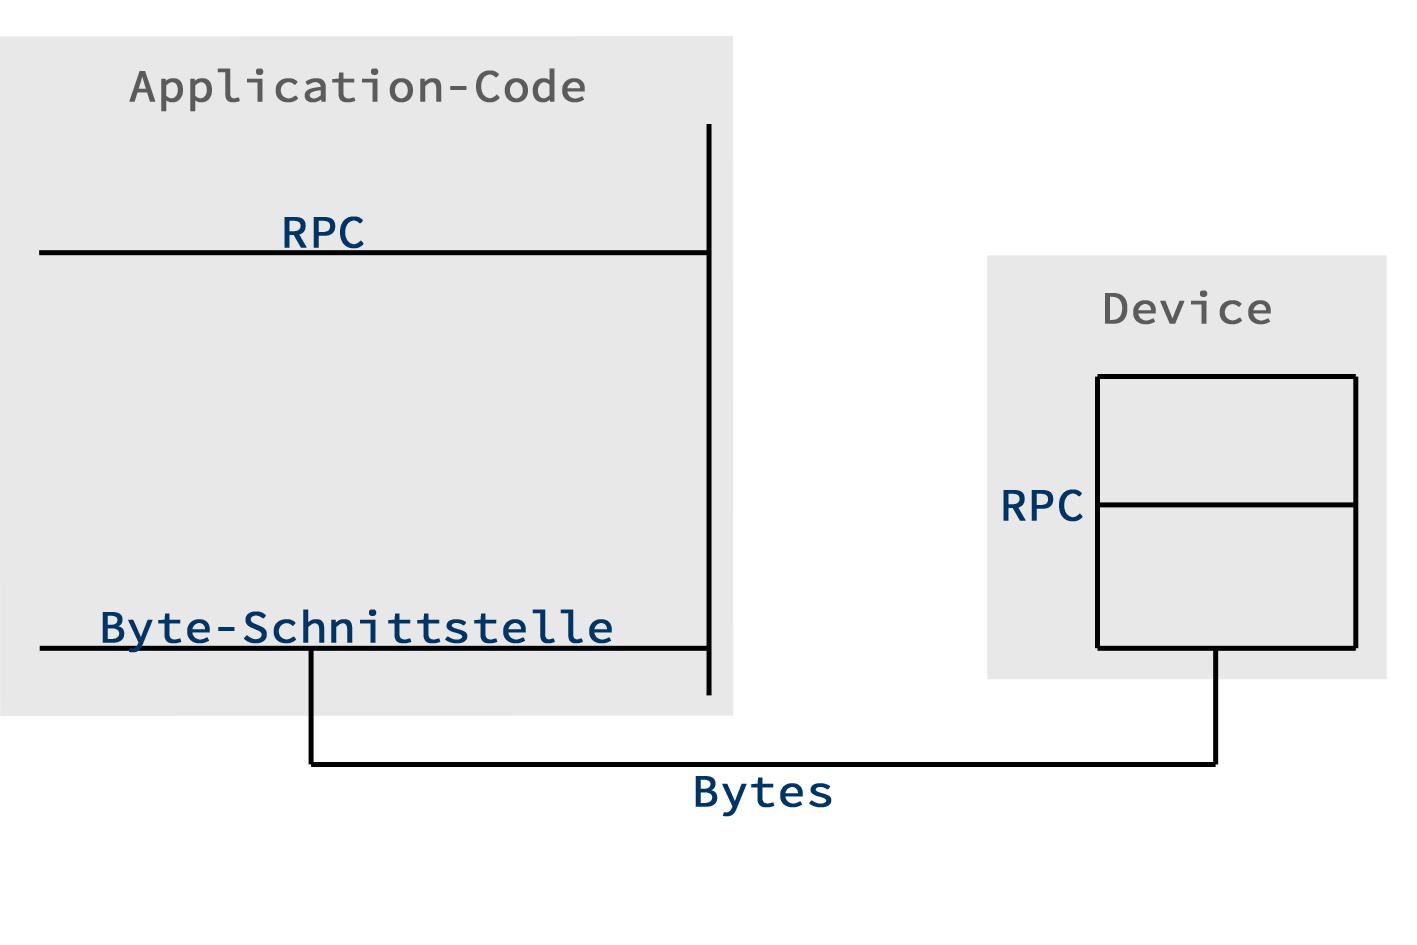
\includegraphics[width=\textwidth]{workfiles/v2_1}
	\end{figure}

	\newpage

	\begin{figure}[h]
		\caption{Hierarchisches Dateisystem}
		\begin{center}
			\tikzstyle{every node}=[anchor=west]
			\begin{tikzpicture}[%
			  grow via three points={one child at (0.5,-0.7) and
			  two children at (0.5,-0.7) and (0.5,-1.4)},
			  edge from parent path={(\tikzparentnode.south) |- (\tikzchildnode.west)}]
			  \node {/}
			    child { node {a}}
			    child { node {b}}
			    child { node {c/}
			      child { node {x}}
			      child { node {y}}
			      child { node {z/}}
			    };
			\end{tikzpicture}
		\end{center}
	\end{figure}

	\begin{figure}[h]
		\caption{Kommunikation zwischen Kernel und Prozess}
		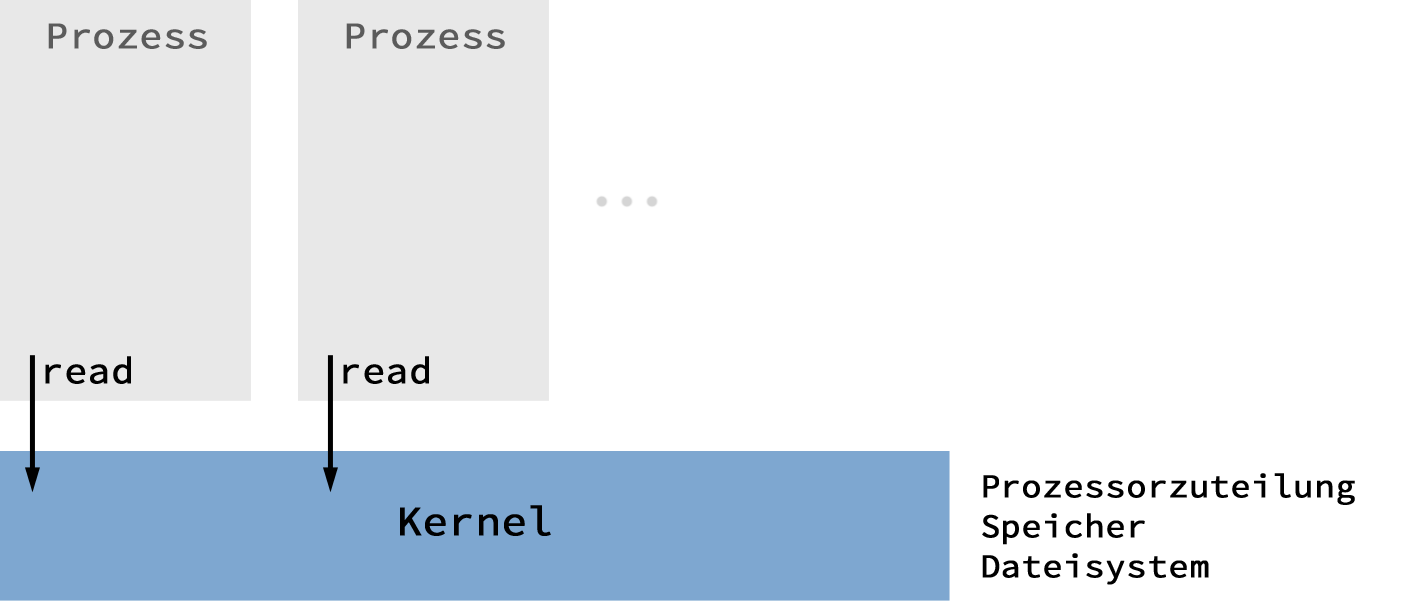
\includegraphics[width=\textwidth]{workfiles/v2_2}
	\end{figure}
	Auch die Shell ist ein Prozess und folgt diesem Kommunikationsschema.\\

	\subsubsection*{Lokaler Dateiaufruf} % (fold)
	\label{ssub:dateiaufrufe}
		
		\lstCcode[Lokaler Dateiufruf]
		\begin{lstlisting}
File *fopen(path)
		\end{lstlisting}

		\begin{figure}[h]
			\caption{Dateiaufruf im Programm}
			
\includegraphics[width=\textwidth]{workfiles/v2_3}
		\end{figure}

		Merkmale des Konzepts
		\begin{itemize}
			\item lokale Aufrufe schneller
			\item andere Prozesse können Datei überschreiben
		\end{itemize}

		\lstCcode[Aufbau einer \texttt{FILE}-Struktur nach \texttt{fopen()}]
		\begin{lstlisting}
f = fopen(path)
f->buf	// Speicher
f->len	// Laenge
f->fd		// File Descriptor
		\end{lstlisting}

	% subsubsection dateiaufrufe (end)

	\subsubsection*{Systemweiter Dateiaufruf} % (fold)
	\label{ssub:systemweiter_dateiaufruf}

		\lstCcode[Systemaufruf]
		\begin{lstlisting}
int open(path)
		\end{lstlisting}

		\begin{itemize}
			\item Systemaufruf, Kernel wird angesprochen
			\item verschiedene Prozesse können nicht gleichzeitig auf das 1. Byte zugreifen
		\end{itemize}
	
	% subsubsection systemweiter_dateiaufruf (end)

	\subsubsection*{Fork und Exec} % (fold)
	\label{ssub:aufruf_von_fork}
	
		\lstCcode[Welcher Prozess bin ich nach dem \texttt{fork()}?]
		\begin{lstlisting}
if(pid = fork()) {
 // parent
} else {
 // child
}
		\end{lstlisting}

		\lstCcode[Weiterführen mit \texttt{exec()}]
		\begin{lstlisting}
if(pid = fork()) {
 // parent
} else {
 // child
 exec();
}
		\end{lstlisting}

	% subsubsection aufruf_von_fork (end)

	\subsubsection*{Fork und Exec am Beispiel von butfirst.sh} % (fold)
	\label{ssub:fork_am_beispiel_von_butfirst_sh}
	
		\lstShell
		\begin{lstlisting}
#!/bin/sh
read
exec doit
		\end{lstlisting}

		\begin{figure}[th]
			\caption{Ablauf von Fork und Exec}
			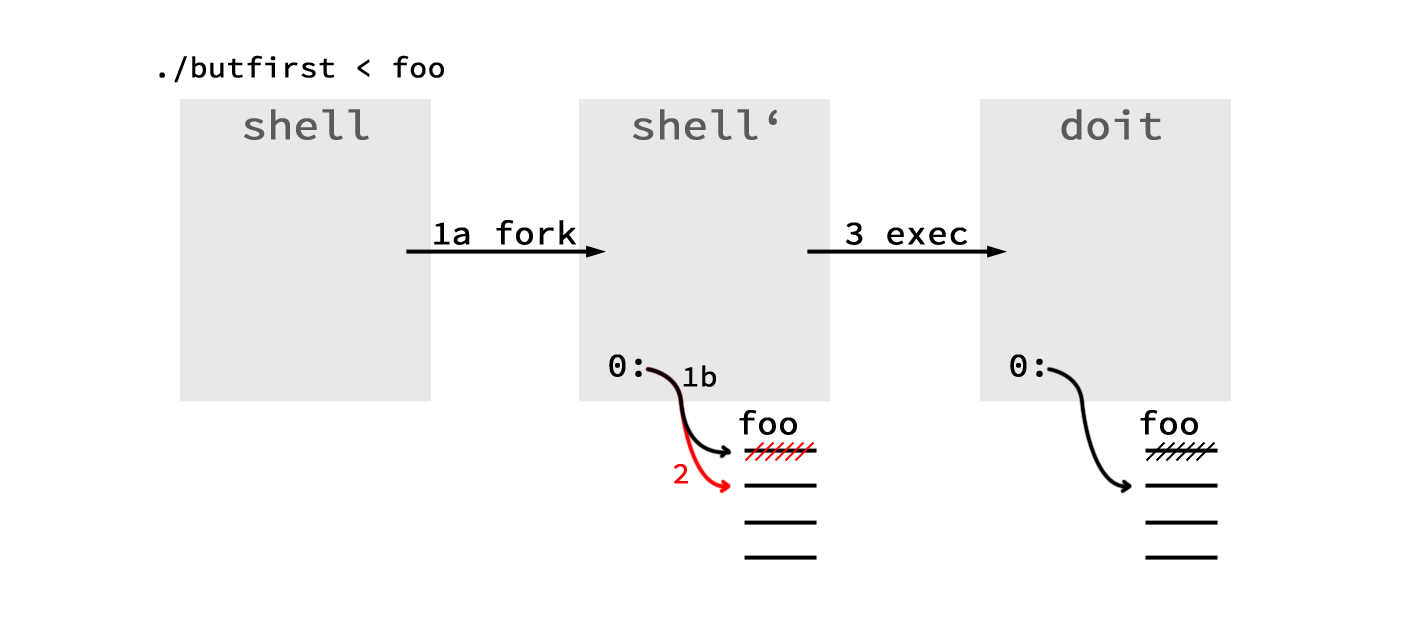
\includegraphics[width=\textwidth]{workfiles/v2_4}
		\end{figure}

	% subsubsection fork_am_beispiel_von_butfirst_sh (end)

	% subsection prozesspipelines_und_glue_languages (end)

	%%%%
	%%%% end V2
	%%%%

	\subsubsection*{Textausgabe in Haskell} % (fold)
	\label{ssub:textausgabe_in_haskell}
	
		\lstHaskell
		\begin{lstlisting}
main = putstrln "Hello World!"
		\end{lstlisting}

		\lstHaskell[Mehrzeilige Ausgabe, Variante 1]
		\begin{lstlisting}
main = putstrln "Hello World!" >> putstrln "Foobar"
		\end{lstlisting}

		\lstHaskell[Mehrzeilige Ausgabe, Variante 2]
		\begin{lstlisting}
main = do {
		putstrln "Hello World!"
		putstrln "Foobar"
	}
		\end{lstlisting}

	% subsubsection textausgabe_in_haskell (end)

	\subsubsection*{Umgebungsvariablen} % (fold)
	\label{ssub:umgebungsvariablen}

		Ausgabe von \texttt{Hello\$USER} ist klar, aber was ist mit \texttt{\$USERHello}?
		\begin{itemize}
			\item gesucht wird nach \texttt{\$USERHello} $\rightarrow$ führt meist zu einem \texttt{not found}
			\item Lösung durch Klammerung: \texttt{\$\{USER\}Hello}
		\end{itemize}

	% subsubsection umgebungsvariablen (end)

	\subsubsection*{Trennzeichen in der Shell} % (fold)
	\label{ssub:trennzeichen_in_der_shell}
	
		Trennzeichen, die in der Varaible \texttt{\$ISF} stehen, werden zur Worttrennung genutzt:
		\lstShell
		\begin{lstlisting}
" \n\t"
		\end{lstlisting}
		Einfaches Ausgeben via \texttt{echo} führt allerdings zu keiner Ausgabe:
		\lstShell
		\begin{lstlisting}
$ echo $IFS
>
		\end{lstlisting}
		Grund: Es sind nur Whitespace-Zeichen, die abgeschnitten werden. Ausgabe als Whitespace möglich (erkennbar an zwei Newlines) über:
		\lstShell
		\begin{lstlisting}
$ echo "$IFS"
>
>
		\end{lstlisting}

	% subsubsection trennzeichen_in_der_shell (end)

	\subsubsection*{Shellübersicht} % (fold)
	\label{ssub:shell_bersicht}
	
		\begin{tabular}{lll}
			bash	&	Bourne Again Shell 	&	in Vorlesung genutzt\\
			sh		&	Bourne Shell 		&	ursrüngliche Shell\\
			csh		&	c Shell 			&	\\
			ksh		&	Korn Shell 			&	
		\end{tabular}

	% subsubsection shell_bersicht (end)

	\subsubsection*{True und False in der Shell} % (fold)
	\label{ssub:true_und_false_in_der_shell}
	
		In der Shell sind auch \texttt{true} und \texttt{false} ausführbare Programme.
		\lstCcode[\texttt{true} als C-Programm]
		\begin{lstlisting}
int main() { return 0; }
		\end{lstlisting}

	% subsubsection true_und_false_in_der_shell (end)

	\subsubsection*{Vorsicht vor deprecated Befehlen} % (fold)
	\label{ssub:vorsicht_vor_deprecated_befehlen}
	
		Veraltete Befehle können Sicherheitsrisiken sein. Beispiel \texttt{gets()}:

		\lstCcode[testpwd.c]
		\begin{lstlisting}
getInp() {
	char buff[1000];
	gets(buff);
}
		\end{lstlisting}
		\begin{figure}[hbtp]
			\caption{Illustrations des gets-Problems}
			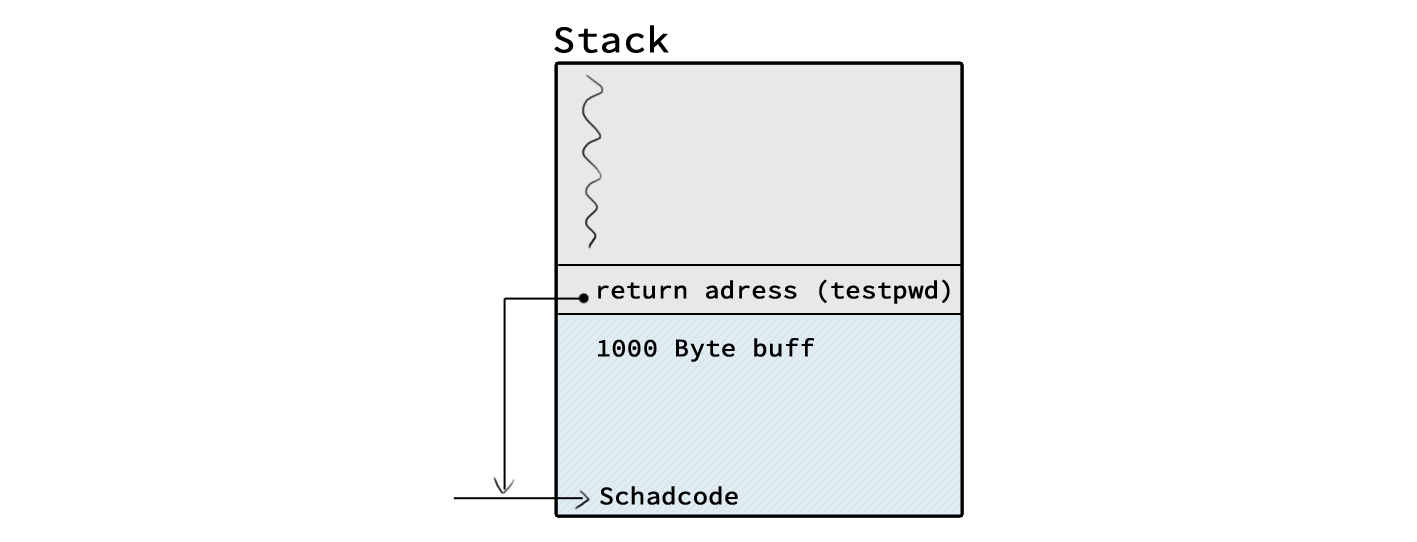
\includegraphics[width=\textwidth]{workfiles/v3_1}
		\end{figure}

	% subsubsection vorsicht_vor_deprecated_befehlen (end)

	\subsubsection*{Dateiumleitungen} % (fold)
	\label{ssub:dateiumleitungen}
	
		\begin{tabular}{ll}
			\texttt{> file}		&	in \texttt{file} leiten	\\
			\texttt{>> file}	&	an \texttt{file} anfügen	\\
			\texttt{< file}		&	aus \texttt{file} lesen	\\
			\texttt{1 > file}	&	File Descriptor 1 leitet in \texttt{file}	\\
			\texttt{2 >\& 1}	&	FD2 leitet in selbes Ziel wie FD 1	\\
			\texttt{FD0}		&	Standardinput	\\
			\texttt{FD1}		&	Standardoutput	\\
			\texttt{FD2}		&	Standarfehlerausgabe	\\
		\end{tabular}

		\begin{flalign*}
			&\text{\texttt{printf("Hello$\backslash$n");}}	\\
			&\qquad\downarrow	\\
			&\text{\texttt{FILE *stdout}}	\\
			&\qquad\downarrow	\\
			&\text{\texttt{write(stdout->fd, stdout->buf, stdout->len);}}
		\end{flalign*}

	% subsubsection dateiumleitungen (end)

	%%%%
	%%%% end V3
	%%%% % 2.-3. VL
		\subsection{Pipes} % (fold)
	\label{sub:pipes}
	
		\begin{figure}[ht]
			\caption{Schematische Darstellung einer (unnamed) Pipe}
			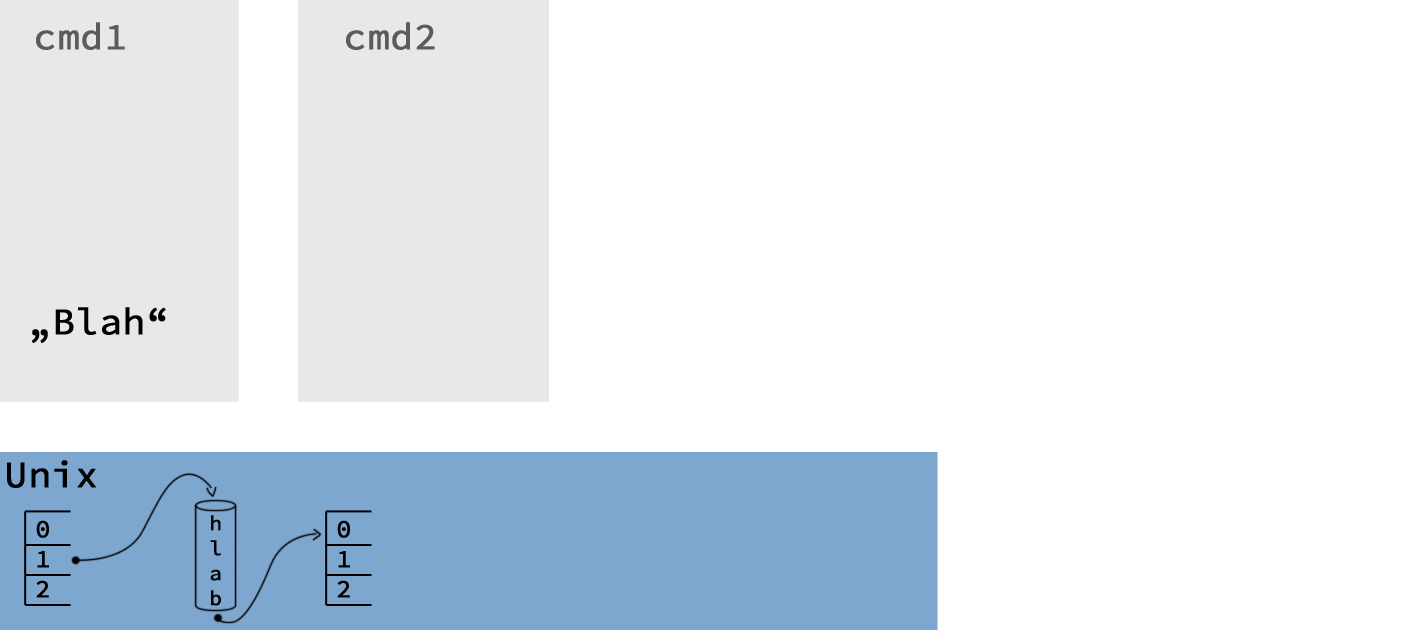
\includegraphics[width=\textwidth]{workfiles/v4_1}
		\end{figure}

		\subsubsection*{Named Pipe} % (fold)
		\label{ssub:named_pipe}

			\lstShell[Variante 1]
			\begin{lstlisting}
cmd filename
cmd2 < filename
			\end{lstlisting}

			\lstShell[Variante 2]
			\begin{lstlisting}
mkfifo filename
cmd filename &
cmd2 < filename
			\end{lstlisting}

		% subsubsection named_pipe (end)

		\subsubsection*{Vorteil Pipes} % (fold)
		\label{ssub:vorteil_pipes}
		
			\begin{itemize}
				\item sequentielle Abarbeitung möglich
				\item 1 arbeitet, 2 muss nicht warten
				\item Prozesssynchronisation
			\end{itemize}

		% subsubsection vorteil_pipes (end)

		\subsubsection*{Analog in Haskell} % (fold)
		\label{ssub:analog_in_haskell}
		
			\lstHaskell
			\begin{lstlisting}
head.(map f3).(map f2).(map f1)[1..]
			\end{lstlisting}

		% subsubsection analog_in_haskell (end)

		\subsection*{Interessantes Pipe-Verhalten} % (fold)
		\label{sub:interessantes_pipe_verhalten}
			
			\subsubsection*{cut} % (fold)
			\label{ssub:cut}

				\lstShell
				\begin{lstlisting}
cut -d " " -f 2
				\end{lstlisting}

				Liefertes das f-te Element (\texttt{-f}), Feldtrennung anhand von \texttt{-d}

			% subsubsection cut (end)

			\subsubsection*{tr} % (fold)
			\label{ssub:tr}
			
				\lstShell
				\begin{lstlisting}
tr [:lower:] [:upper:]
				\end{lstlisting}

				Translate übersetzt Zeichen, hier von lower nach upper.

			% subsubsection tr (end)

			\subsubsection*{In Kombination} % (fold)
			\label{ssub:in_kombination}
			
				\lstShell
				\begin{lstlisting}
cut -d " " -f 2 | tr [:lower:] [:upper:]
				\end{lstlisting}

				Läuft nicht wie gewünscht, aber
			
				\lstShell
				\begin{lstlisting}
cut -d " " -f 2 < foo| tr [:lower:] [:upper:]
				\end{lstlisting}

				schon. Was ist das Problem?

				\begin{itemize}
					\item Pufferung im Prozess
					\item wenn FD aus Terminal $\rightarrow$ Zeilenpufferung
					\item wenn FD kein Terminal $\rightarrow$ Blockpufferung
				\end{itemize}

				Lösung daher: Nutzung eines Pseudo-Terminals

				\lstShell
				\begin{lstlisting}
/dev/pty
				\end{lstlisting}

				\begin{figure}[hbtp]
					\caption{pty, Pseudo-Terminal, Schema}
					
\includegraphics[width=\textwidth]{workfiles/v4_2}
				\end{figure}

				\begin{figure}[hbtp]
					
\includegraphics[width=\textwidth]{workfiles/v5_1}
				\end{figure}

				Problem der Blogpufferung: siehe letzte Vorlesung

			% subsubsection in_kombination (end)


	%%%%
	%%%% end V4
	%%%%
	%%%% V5
	%%%%
		% subsection interessantes_pipe_verhalten (end)

		\subsection*{Kommunikation vo Pipes in "`Echtzeit"'} % (fold)
		\label{sub:kommunikation_vo_pipes_in_}

			$\;$
			\begin{figure}[phbt]
				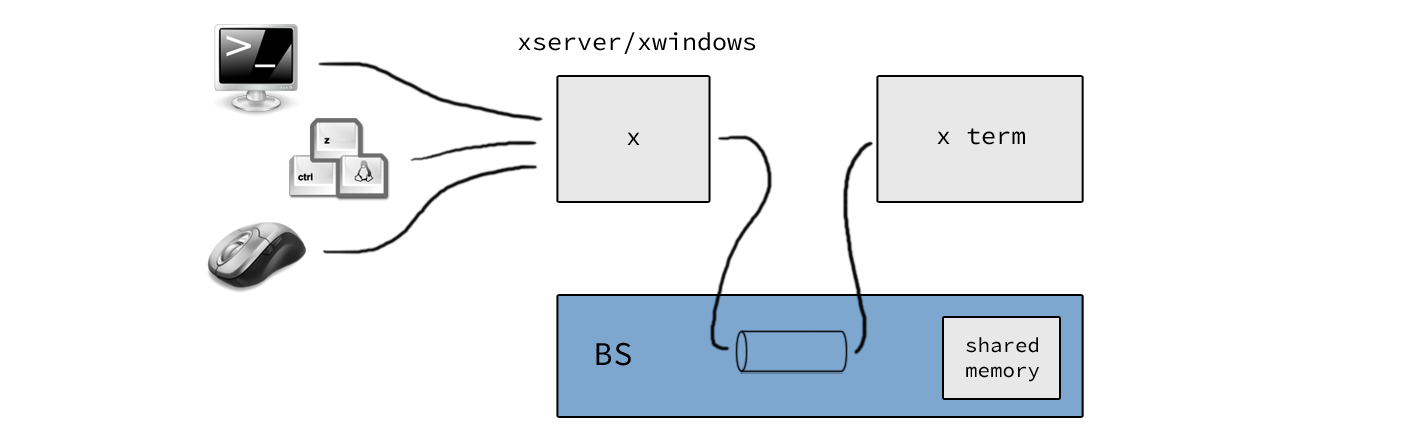
\includegraphics[width=\textwidth]{workfiles/v5_2}
			\end{figure}

			Allerdings keine tatsächliche Echtezit, da unter Unix keine Zeitgarantien exisiteren.
			Harte Echtzeit gibt es bspw. unter OS 9, VxWorks oder PSOS.\\
			Möglich auch durch verteilte Systeme

			\begin{figure}[hbtp]
				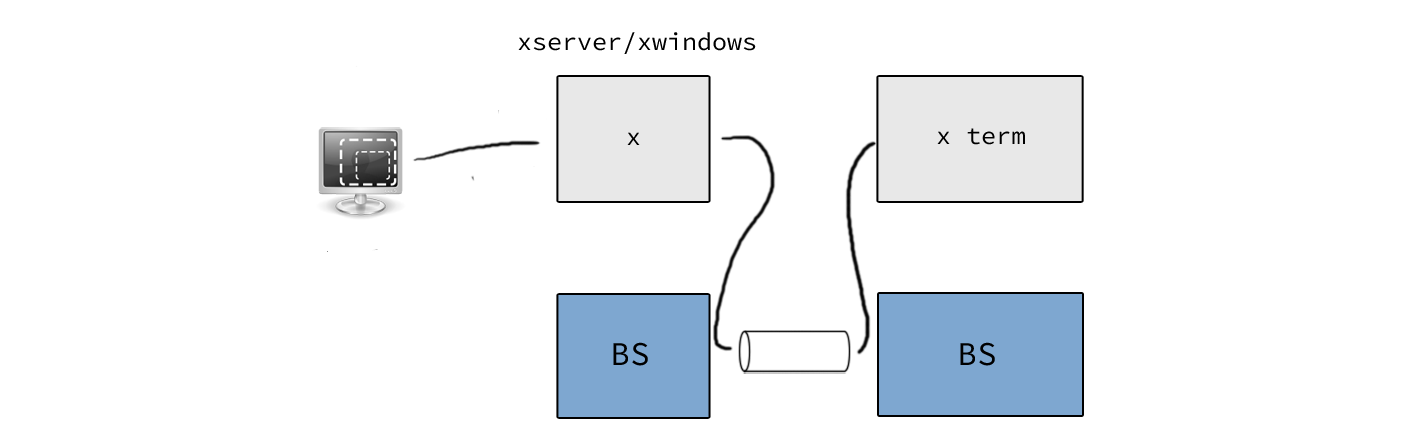
\includegraphics[width=\textwidth]{workfiles/v5_3}
			\end{figure}
		
		% subsection kommunikation_vo_pipes_in_ (end)

	% subsection pipes (end) 		% 4.-5. VL
		\subsection{Bash-Skripte und weitere Tools} % (fold)
	\label{sub:bash_skripte_und_weitere_tools}

		\lstBash[Rückgabewert des letzten Programms]
		\begin{lstlisting}
$?
		\end{lstlisting}
		\lstBash[direkte Ausgabe bis zum nächsten \texttt{eof}]
		\begin{lstlisting}
cat << 'eof'
		\end{lstlisting}
		\lstBash[erst Auswertung, dann Ausgabe]
		\begin{lstlisting}
cat << eof
		\end{lstlisting}
		Technik bereits vom Interpreter bekannt:
		\lstBash
		\begin{lstlisting}
cat > testing.c << eof
# C-Code mit Expressions
eof
		\end{lstlisting}

		\subsubsection*{Kontrollmechanismen} % (fold)
		\label{ssub:kontrollmechanismen}
		
			\lstBash[Einfache Verzeweigungen]
			\begin{lstlisting}
if <cmd> then
	<cmd>
elif <cmd> then
	<cmd>
else
	<cmd>
fi
			\end{lstlisting}
			\lstBash[\texttt{case}-Verzweigung]
			\begin{lstlisting}
case <var> in
	(Muster) <cmd> ;;
	(Muster) <cmd> ;;
esac
			\end{lstlisting}
			Hierbei ist als \texttt{Muster} eine vereinfachte Form von RegEx möglich.
			\lstBash[\texttt{while}-Schleife]
			\begin{lstlisting}
while <cmd>
do
	<cmd>
done
			\end{lstlisting}
			\lstBash[\texttt{unitl}-Schleife]
			\begin{lstlisting}
until <cmd>
do
	<cmd>
done
			\end{lstlisting}
			\lstBash[\texttt{for}-Schleife]
			\begin{lstlisting}
for <var> in w1 w2 w3 ...
do
	<cmd>
done
			\end{lstlisting}
		% subsubsection kontrollmechanismen (end)

		\subsubsection*{Beispiele Kontrollmechanismen} % (fold)
		\label{ssub:beispiele_kontrollmechanismen}

			\lstBash[Ausgabe Verzeichnisinhalt]
			\begin{lstlisting}
	for i in *; do echo $i; done
			\end{lstlisting}
			\lstBash
			\begin{lstlisting}
	for((i=1;i<200;i++)) do ... done
			\end{lstlisting}
			\lstBash[erstellt einfaches Auswahlmenü mit Verzeichnisinhalt]
			\begin{lstlisting}
	select i in *; do echo $i; done
			\end{lstlisting}
		
		% subsubsection beispiele_kontrollmechanismen (end)

		\subsubsection*{Funktionen und Argumente} % (fold)
		\label{ssub:funktionen_und_argumente}
		
			\lstBash[Variablenklammer bleibt leer]
			\begin{lstlisting}
func() {
	...
}
			\end{lstlisting}
			\lstBash
			\begin{lstlisting}
$0 $1 $2 ...
			\end{lstlisting}
			Wird ein \texttt{shift} auf den Variablen ausgeführt, ergibt sich folgendes Schema\\
			\begin{tikzpicture}
				\matrix (m) [matrix of math nodes,row sep=1.5em,column sep=2em,minimum width=2em]
				{
					\texttt{\$0} & \texttt{\$1} & \texttt{\$2} & ... & & \texttt{\$8} & \texttt{\$9} \\
					\texttt{\$0} & \texttt{\$1} &  & ... & \texttt{\$7} & \texttt{\$8} & \\
				};
				\path[->]
					(m-1-1) edge (m-2-1)
					(m-1-3) edge (m-2-2)
					(m-1-6) edge (m-2-5)
					(m-1-7) edge (m-2-6);
			\end{tikzpicture}

		% subsubsection funktionen_und_argumente (end)

		\subsubsection*{Textverarbeitung} % (fold)
		\label{ssub:textverarbeitung}
		
		\lstShell[Werte zuweisen mittels \texttt{read}]
		\begin{lstlisting}
$ read a b c
> 1 2 3 4 5
		\end{lstlisting}
		\lstShell[Ausgabe gespeicherter Werte]
		\begin{lstlisting}
$ echo $a $b -- $c
> 1 2 -- 3 4 5
		\end{lstlisting}
		\lstShell[Formatierte Strings]
		\begin{lstlisting}
$ printf "%f\n" 1e-6
		\end{lstlisting}
		% subsubsection textverarbeitung (end)

		\subsubsection*{Streameditor \texttt{sed}} % (fold)
		\label{ssub:streameditor_sed}
		
		\lstShell[liefert Zeile 1 und 1000]
		\begin{lstlisting}
$ sed -n -e'1p -e'1000p' < data.csv
		\end{lstlisting}
		\texttt{sed} ist sehr leistungsfähig für die Zielenverabeitung von Daten

		% subsubsection streameditor_sed (end)

		\subsubsection*{Aho-Weinberg-Kernigton \texttt{awk}} % (fold)
		\label{ssub:aho_weinberg_kernigton_awk}
		
		\lstShell
		\begin{lstlisting}
awk  '/Muster/{Anweisung}'
awk '/^\#/{print $2}'
awk '{print $2}'      # Ausfuehrung immer
awk 'NR==3{...}'       # Zeile 3
awk 'NR<2&&/^\#/{...}'  # vor Zeile 2 und das Muster treffend
		\end{lstlisting}

	%%%%
	%%%% end V5
	%%%%
	%%%% V6
	%%%%

			Im Allgemeinen exisitiert in Unix folgende Vorstellung der Datenverarbeitung:\\

			% Define block styles
			\tikzstyle{box} = [rectangle, draw, text centered, minimum height=2em]
			\tikzstyle{emp} = [rectangle, text centered, minimum height=2em]
			\tikzstyle{line} = [draw, -latex']
			\begin{tikzpicture}[node distance = 1.5cm, auto]
			    % Place nodes
			    \node [emp] (0a) {};
			    \node [emp, right of=0a] (0b) {};
			    \node [box, above right of=0b] (1) {};
			    \node [box, below right of=0b] (2) {};
			    \node [box, right of=1] (3) {};
			    \node [box, below right of=3] (4) {};
			    \node [box, right of=4] (5) {awk};
			    \node [box, right of=5] (6) {};
			    \node [emp, right of=6] (f) {};
				
			    % Draw edges
				\path [line] (0a) -- (0b);
				\path [line] (0b) -- (1);
				\path [line] (0b) -- (2);
				\path [line] (1) -- (3);
				\path [line] (2) -- (4);
				\path [line] (3) -- (4);
				\path [line] (4) -- (5);
				\path [line] (5) -- (6);
				\path [line] (6) -- (f);
			\end{tikzpicture}

			\lstBash[awk-File]
			\begin{lstlisting}
pattern {action} # jede Eingabezeile wird von oben
pattern {action} # nach unten geprueft
...
			\end{lstlisting}

		% subsubsection aho_weinberg_kernigton_awk (end)

		\subsubsection*{Weiterer Bezug auf das Sensorbeispiel} % (fold)
		\label{ssub:weiterer_bezug_auf_das_sensorbeispiel}

			\begin{flalign*}
				 \left.\begin{array}{rcl}
				 	-2g & \approx & 0\\
				 	0g & \approx & 2047\\
				 	2g & \approx & 4095\\
				 \end{array}\right\}x_{raw}\\
				 \rightarrow\text{12bit Sensorauflösung}
			\end{flalign*}
			Gewünscht ist dafür eine Zentrierung
			\begin{flalign*}
				x_{cooked}\sim N\left(\mu=0,\sigma=1\right)
			\end{flalign*}
			Dafür werden folgende Werte erfasst
			\begin{flalign*}
				\text{\texttt{x[i]}}=\sum_{j=1}^nx_j\\
				\text{\texttt{xx[i]}}=\sum_{j=1}^nx_j^2
			\end{flalign*}
			Wie realisiert \texttt{swk} Felder? Balancierte Bäume.\\
			\texttt{x[i]} - i ist Index des Baumblattes\\
			\texttt{x[i,j]} - i\^{}@j ist Index des Blattes\\

			Vorsicht: Trennzeichen sollte nicht in Indexstring vorkommen.\\

			\lstShell[Anwendung von \texttt{prog} auf übergebene Dateien]
			\begin{lstlisting}
$ awk -f prog file1 file2
			\end{lstlisting}
			Hierbei wird jede Datei zeilenweise verarbeitet. Für das Programm existieren
			zwei Zähler:\\
			NR - aktuelle Zeilennummer insgesamt\\
			FNR - aktuelle Zeilennummer in einer Datei\\

			Formeln für \texttt{rescale.awk}
			\begin{flalign*}
				x &= \frac{x_{raw}-\mu}{\sigma}\\
				r &= \sqrt{x^2+y^2+z^2}
			\end{flalign*}

			Summieren von großen Zahlenmengen ist bspw. durch Kahan-Summing gut lösbar.

		
		% subsubsection weiterer_bezug_auf_das_sensorbeispiel (end)
	
	% subsection bash_skripte_und_weitere_tools (end)

	%%%%
	%%%% end V6
	%%%% 		% 5.-6. VL
% section shellprogrammierung (end)

\clearpage
\section{Monaden und Interaktive Programme} % (fold)
\label{sec:monaden_und_interaktive_programme}
		%%%
	%%% V7
	%%%

	\subsection{Polymorphismus in Haskell} % (fold)
	\label{sub:polymorphismus_in_haskell}
		\begin{itemize}
			\item parametrischen über Typvariablen
			\item ad-hoc übr Typklassen
		\end{itemize}

		\subsubsection*{Unterschied} % (fold)
		\label{ssub:unterschied}
			\begin{tabular}{lcp{8cm}}
				ad-hoc & $\equiv$ & derselbe Name für unterschiedliche Algorithmen\\
				parametrischer & $\equiv$ & derselbe Name für den gleichen Algorithmus, also ein Algorithmus für alle Typen
			\end{tabular}
		% subsubsection unterschied (end)

		\subsubsection*{Beispiel parametrischer Polymorphismus} % (fold)
		\label{ssub:beispiel_parametrischer_polymorphismus}
			\lstHaskell
			\begin{lstlisting}
length :: [a] -> Int
length [] = 0
length (_:l) = 1 + length l
			\end{lstlisting}
		% subsubsection beispiel_parametrischer_polymorphismus (end)
	% subsection polymorphismus_in_haskell (end)

	\subsection{Weltveränderung} % (fold)
	\label{sub:weltveraenderung}
		\lstHaskell
		\begin{lstlisting}[morekeywords={sgetLine}]
sgetLine :: IO String
		\end{lstlisting}
		\lstHaskell
		\begin{lstlisting}
p :: IO a
q :: IO b
p >> q :: IO b
p >> q = \w -> let (a,w') = p w
                   (b,w'') = q w'
               in (b,w'')
		\end{lstlisting}
		Was nichts anderes ist als
		\lstHaskell
		\begin{lstlisting}
p >> q = q.snd.p
		\end{lstlisting}
		\lstHaskell
		\begin{lstlisting}
getChar :: IO Char
putChar :: Char -> IO ()
		\end{lstlisting}
		\lstHaskell
		\begin{lstlisting}
(>>=) :: IO a -> (a -> IO b) -> IO b
p :: IO a
f :: a -> IO a

p >>= f :: IO b
p >>= f = \w -> let (a,w') = p w
                    (b,w'') = w'
                in (b,w'')
		\end{lstlisting}
		\lstHaskell
		\begin{lstlisting}
do {a; b} == do a
                b
		\end{lstlisting}
		\lstHaskell
		\begin{lstlisting}
{f;g;}h; != f;{g;h;}
		\end{lstlisting}
		\lstHaskell
		\begin{lstlisting}
data Ampel = Rot
           | Gelb
           | Gruen
data Tree a = Nil |
              Node a Tree Tree
		\end{lstlisting}
		\lstHaskell
		\begin{lstlisting}[mathescape]
IO (\w -> ((),w)) $\equiv$ IO \$ \w -> ((),w)
		\end{lstlisting}

		%%%
		%%% end V7
		%%%
		%%%
		%%% V8
		%%%

		\lstHaskell
		\begin{lstlisting}
-- generisch
MState s a

-- konkret
MS (\x -> (x,17))

-- und damit Typ
MState s Int
		\end{lstlisting}

		\lstHaskell
		\begin{lstlisting}
bla = MS (\x -> (x,17))
(runMState bla) :: s -> (s,Int)
		\end{lstlisting}

		\lstHaskell[Mitzählen von \texttt{getc} als Aktion, aber keine Auslieferung]
		\begin{lstlisting}
getc = \s -> (s+1,s)
		\end{lstlisting}

		\lstHaskell[Zähler zurücksetzen]
		\begin{lstlisting}
put = \s' -> MS $ \s -> (s',s)
		\end{lstlisting}

		\lstHaskell[Kurzform vereinfacht Nutzung und Schachtelung]
		\begin{lstlisting}
-- Langform
MState s a

-- Kurzform
m a

-- Nutzung
instance Monad m where
		\end{lstlisting}

		\lstHaskell[detaillierte Aufschlüsselung anhand von \texttt{get >>= put}]
		\begin{lstlisting}
get = MS (\s -> (s,s))
put = \s' -> MS (\s -> (s',s))
runMState (MS f) = f

get >>= put

MS (\s -> let (s',a) = runMState (MS (\s -> (s,s))) s
          in runMState (put s) s')
MS (\s -> let (s',a) = (\s -> (s,s)) s
          in runMState (put s) s')
MS (\s -> let (s',a) = (s,s)
          in runMState (put s) s')
MS (\s -> runMState (put s) s)
MS (\s -> runMState (MS (\s -> (s,s))) s)
MS (\s -> (\s -> (s,s)) s)
MS (\s -> (s,s))
		\end{lstlisting}
		
		\begin{figure}[ht]
			\caption{Realisierung Verkettung äußerer mit innerer Monade}
			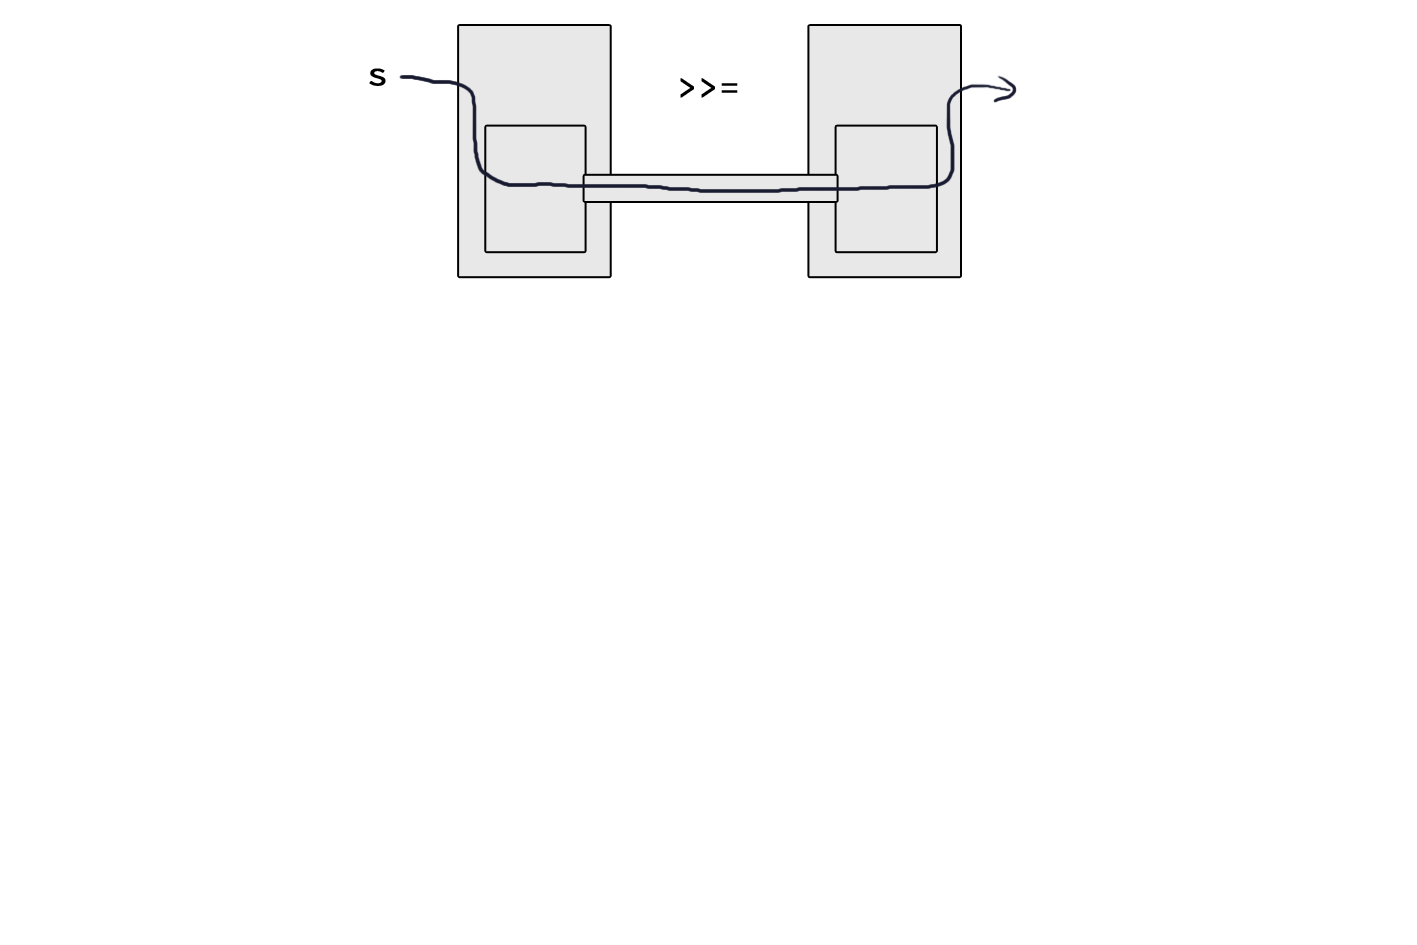
\includegraphics[width=\textwidth]{workfiles/v8_1}
		\end{figure}

	% subsection weltveraenderung (end)

	%%%
	%%% end V8
	%%% % 7.-10. VL
% section monaden_und_interaktive_programme (end)

\clearpage
\appendix
\section{Übungen} % (fold)
\label{sec:uebungen}
		\subsection{Übung 1} % (fold)
	\label{sub:uebung_1}
	Die behandelten Shell-Programme und Funktionen sind meist nur lose augelistet. Genaue Informationen
	lassen sich über die Man-Pages erfahren.

	\lstShell[print working directory]
	\begin{lstlisting}
$ pwd
	\end{lstlisting}

	\lstShell[Weitere Shell-Programme zur Dateiverwaltung]
	\begin{lstlisting}
cd, ls, exit, mkdir, rm, touch, cp, mv
	\end{lstlisting}

	\subsubsection*{Verzeichnisse im Unix-Dateisystem} % (fold)
	\label{ssub:verzeichnisse_im_unix_dateisystem}

	\begin{tabular}{ll}
		\texttt{/tmp} 			& Temporär\\
		\texttt{/dev} 			& devices\\
		\texttt{/usr} 			& unix system resources\\
		\texttt{(usr/local)} 	& Programme (nicht immer vorhanden)\\
		\texttt{/bin} 			& Binärdaten\\
		\texttt{/home} 			& \multirow{2}{*}{User data}\\
		\texttt{/users} 		&\\
		\texttt{/dev/hda}		& \multirow{2}{*}{Drives}\\
		\texttt{/dev/sda}		&\\
		\texttt{dev/tty}		& Terminals\\
		\texttt{dev/null}		& Garbage
	\end{tabular}

	% subsubsection verzeichnisse_im_unix_dateisystem (end)

	\subsubsection*{Verzeichnisnavigation} % (fold)
	\label{ssub:verzeichnisnavigation}

	Pfade, die mit einem \texttt{/} beginnen, sind absolut, alle anderen sind relativ.
	
	\lstShell
	\begin{lstlisting}
$ cd ~  # home directory
$ cd -  # go back
$ cd .. # go up
	\end{lstlisting}

	% subsubsection verzeichnisnavigation (end)

	\lstShell[Aufruf Man-Page (Handbuch) von \texttt{myCommand}]
	\begin{lstlisting}
$ man myCommand
	\end{lstlisting}

	\lstShell[Suche nach \texttt{term}]
	\begin{lstlisting}
$ apropos term
	\end{lstlisting}

	\lstShell[word count in \texttt{file} (auch mehr als Worte)]
	\begin{lstlisting}
$ wc file
	\end{lstlisting}

	\subsubsection*{Dateiberechtigungen} % (fold)
	\label{ssub:dateiberechtigungen}
	
	\begin{tabular}{lllll}
		\texttt{d} 	& \texttt{rwx} 	& \texttt{rwx} 	& \texttt{rwx} 	& \texttt{n}\\
		Typ			& user 			& group 		& other 		& Verzeichnisanzahl
	\end{tabular}\\

	Dabei kann der Typ folgendes sein:

	\begin{tabular}{ll}
		\texttt{d} 	& Directory\\
		\texttt{l} 	& Link\\
		\texttt{p} 	& named Pipe\\
		\texttt{-} 	& File\\
		\texttt{c} 	& Character Device\\
		\texttt{b} 	& Block Device
	\end{tabular}

	% subsubsection dateiberechtigungen (end)

	\subsubsection*{Dateilinks erstellen} % (fold)
	\label{ssub:dateilinks_erstellen}
	
	\begin{figure}[hp]
		\caption{Hartlink über \texttt{ln}}
		
\includegraphics[width=\textwidth]{workfiles/u1_1}
	\end{figure}
	
	\begin{figure}[hp]
		\caption{Softlink über \texttt{ln -s}}
		
\includegraphics[width=\textwidth]{workfiles/u1_2}
	\end{figure}

	Löscht man \texttt{Original} kann über \texttt{Kopie} noch auf die Datei zugegriffen werden, ein
	Aufruf von \texttt{Softlink} führt allerdings zu Fehlern.

	% subsubsection dateilinks_erstellen (end)

	\subsubsection*{Dateisysteme} % (fold)
	\label{ssub:dateisysteme}
	
	\lstShell[Ein-/Aushängen von Dateisystemen]
	\begin{lstlisting}
$ mount
$ umount
	\end{lstlisting}

	\lstShell[Speicherverbrauch anzeigen]
	\begin{lstlisting}
$ du	# Festplattenplatzverbrauch in Byte
$ df	# liefert zusaetzliche Details
	\end{lstlisting}

	\lstShell[Ändern von Dateiberechtigungen]
	\begin{lstlisting}
$ chmod u=rwx file
$ chmod u-r file
$ chmod u+r file
$ chmod 600 file
	\end{lstlisting}
	
	Bei obiger Darstellung ist \texttt{u} die Kennzeichnung für den aktuellen User, möglich ist auch
	\texttt{g} (Group), \texttt{o} (other) oder \texttt{a} (alle).

	Per Zuweisungen können alle	Permutationen von \texttt{rwx} vergeben werden. Oder per \texttt{-/+} einzelne
	Rechte bearbeitet werden.

	Eine direkte Angaabe als Zahlwert ist ebenfalls möglich. Für jede Nutzerklasse bildet man die Summe
	aus read (4), write (2) und execute (1).

	\lstShell[Ändern von Dateibesitzern]
	\begin{lstlisting}
$ chown user file
$ chown user:group file
	\end{lstlisting}

	% subsubsection dateisysteme (end)

	\subsubsection*{Wildcards in der Shell} % (fold)
	\label{ssub:wildcards_in_der_shell}

	\begin{tabular}{ll}
		\texttt{*} 	& beliebige Zeichenfolge\\
		\texttt{?} 	& beliebiges Zeichen\\
		\texttt{[abcD]} 	& \multirow{2}{*}{\underline{ein} Zeichen aus der Gruppe}\\
		\texttt{[a-z]} 	&\\
		\texttt{\{a,b\}} 	& Aufzählung von Pattern\\
	\end{tabular}

	% subsubsection wildcards_in_der_shell (end)

	% subsection uebung_1 (end) % 1. Ub
		\subsection{Übung 2} % (fold)
	\label{sub:uebung_2}

		\lstShell[ohne versteckte Dateien]
		\begin{lstlisting}
$ du -s * | sort -n -r
		\end{lstlisting}

		\lstShell[alle Dateien]
		\begin{lstlisting}
$ du -d 1 | sort -n -r
		\end{lstlisting}

		\lstShell[Filter]
		\begin{lstlisting}
cat, cut, tr, wc, more, sort, uniq, grep
		\end{lstlisting}

		\lstShell
		\begin{lstlisting}
grep [optionen] suchstring [dateien]
		\end{lstlisting}

		\lstShell[Reguläre Ausdrücke]
		\begin{lstlisting}
\         # Escapezeichen

## Zeichen
[AaBbCc]  # 1 Zeichen muss treffen
[a-z]
[^a-z]    # alles außer...

# Position/Gruppierung
^bar      # Zeilenanfang
\<foo\>   # Wortanfang/Wortende
\(\)      # Zusammenfassung
t1|t2     # Alternativen

## Multiplikatoren
.         # beliebiges Zeichen
.+        # min. 1 mal
.*        # beliebig oft
.?        # 0 oder 1 mal
.{n}      # n-fache Wiederholung
.{n,m}    # von n bis m
.{n,}     # min n mal
		\end{lstlisting}

		\lstShell[\texttt{sed}]
		\begin{lstlisting}
sed "s/welt/neue_welt/"
# sed "optionen1/pattern/ersetzung/optionen2"
		\end{lstlisting}
		Dabei kann \texttt{optionen2} z.B eines der Folgenden sein

		\lstShell
		\begin{lstlisting}
i  # ignore case
g  # global; für ganze Eingabe
		\end{lstlisting}

		\subsubsection{Shellskript} % (fold)
		\label{ssub:shellskript}

			\lstBash[1. Zeile]
			\begin{lstlisting}
#!/bin/bash
			\end{lstlisting}

			\lstBash[Nutzung von Parametern]
			\begin{lstlisting}
$#         # Anzahl Parameter
$1 ... $n  # Parameter n
$*         # alle Parameter als ein String
$@         # einlesen als Array
$0         # Programmname
$?         # Rückgabe letztes Shell-Kommando
			\end{lstlisting}

			\lstBash[Parameter von \texttt{test}]
			\begin{lstlisting}
-f  # Pfad
-e  # exists
-r  # Leserechte
-h  # Symbollink
-d  # Verzeichnis
!   # Negation
-z  # Länge Zeichenkette 0
-n  # Länge Zeichenkette > 0
			\end{lstlisting}

			\lstBash[\texttt{test}-Beispiele]
			\begin{lstlisting}
1 -lt 2  # 1 kleiner 2 ?
         # le, gt, ge, ne, eq
zk1 = zk2  # gleich?
zk1 != zk2 # ungleich?
			\end{lstlisting}

			\lstBash[Fallunterscheidung]
			\begin{lstlisting}
case $1 in
	-a)
		echo
		;;
	-b|-c)
		echo
		;;
	-*)
		echo
		;;
esac
			\end{lstlisting}
			Weitere Schleifenmöglichkeiten sind \texttt{for}, \texttt{while} und \texttt{until}
		
		% subsubsection shellskript (end)

	% subsection uebung_2 (end) % 2. Ub
		\subsection{Übung 3} % (fold)
	\label{sub:_ubung_3}
	
		\lstBash[Arrays in Shellskripten]
		\begin{lstlisting}
array=(red green blue yellow)
directory=`ls`
$array       # 1. Element
$array[0]    # gezielter Zugriff
${#array[*]} # Array-Länge
		\end{lstlisting}

		\lstShell[AWK]
		\begin{lstlisting}
$ awk <pattern> {<command>}
		\end{lstlisting}

	% subsection _ubung_3 (end) % 2. Ub
% section uebungen (end)


\end{document}

% http://tex.stackexchange.com/questions/40682/define-a-new-caption-in-a-listing-environment
% http://www.golatex.de/verschiedene-beschriftungen-mit-listing-t3880.html